\documentclass{article}
\usepackage{graphicx}
\usepackage{caption}
\usepackage{booktabs}
\usepackage{amssymb}
\usepackage{amsmath}
\usepackage[dvipsnames]{xcolor}
\usepackage[T1]{fontenc}
\usepackage[utf8]{inputenc}
\usepackage{subcaption} 
\usepackage{float}
\usepackage{geometry}
\geometry{margin=1in}
\usepackage{graphicx}
\usepackage{babel}
\usepackage{animate}
\usepackage{hyphenat}
\usepackage{url} 

\title{Sprawozdanie z laboratorium 4''}
\author{Hubert Miklas}
\date{08-04-2025}

\begin{document}

\maketitle

\section{Wstęp}

Tematem laboratorium 4'' była kontynuacja aproksymacji i interpolacji.

\section{Zadania}

\section*{Zadanie 1}

Obliczyć 4–5 współczynników aproksymacji funkcji $|x|$ w przedziale $[-1,1]$ wielomianami Czebyszewa. Obliczyć błąd aproksymacji w równoodległych punktach z odstępem 0.2, poczynając od punktu $-0.8$. Narysować na papierze kratkowanym funkcję aproksymowaną i aproksymującą.

\section*{Zadanie 2}

W eksperymencie uzyskano następujące dane dwuwymiarowe $(x,y)$:
\[
(0.0, 0.0),\quad (0.5, 1.6),\quad (1.0, 2.0),\quad (6.0, 2.0),\quad (7.0, 1.5),\quad (9.0, 0.0).
\]
Chcielibyśmy wykonać interpolację danych gładką krzywą celem znalezienia rozsądnych wartości $y$ dla wartości $x$ pomiędzy punktami, w których wykonano pomiary.

\begin{enumerate}
    \item[(a)] Proszę określić wielomian stopnia piątego, który interpoluje podane dane i narysować wykres wielomianu w zakresie od 0 do 9.
    \item[(b)] Proszę obliczyć funkcję sklejaną stopnia trzeciego, która interpoluje podane dane i narysować wykres w tymże zakresie.
    \item[(c)] Proszę obliczyć funkcję interpolującą dla tychże danych przy pomocy wielomianów Czebyszewa i zrobić wykres w tymże zakresie.
    \item[(d)] Która z wyżej obliczonych funkcji interpolujących daje lepsze wyniki pomiędzy zadanymi punktami? Proszę objaśnić, dlaczego ww. funkcje tak się zachowują.
\end{enumerate}


\section*{Zadanie 1}

Mamy kolejne wielomiany Czebyszewa \cite{wiki:Chebyshev_polynomials}:

\begin{align*}
    T_{0}(x) = 1 \\
    T_{1}(x) = x \\
    T_{2}(x) = 2x^2 - 1 \\
    T_{3}(x) = 4x^3 - 3x \\
    T_{4}(x) = 8x^4 -  8x^2 + 1
\end{align*}

Na podstawie wzoru aproksymacyjnego Czebyszewa \cite{wiki:Chebyshev_polynomials, Funika}, możemy obliczyć całki:

Funkcję $f(x)$ aproksymujemy szeregiem:
\begin{equation}
    f(x) = \sum_{i=0}^n c_{i} T_{i}(x)    
    \label{chebyshev}
\end{equation}
Gdzie współczynniki $c_i$ można obliczyć ze wzoru:

\begin{align*}
    c_0 = \frac{1}{\pi} \int_{-1}^{1} \frac{f(x)T_k(x)} {\sqrt{1 - x^2}} \, dx. \\
c_k = \frac{2}{\pi} \int_{-1}^{1} \frac{f(x) T_k(x)}{\sqrt{1 - x^2}} \, dx \quad \text{dla } k > 0,  
\end{align*}

Możemy zatem obliczyć te całki:
\begin{align*}
c_0 &= \frac{1}{\pi} \int_{-1}^{1} \frac{f(x) \cdot 1}{\sqrt{1 - x^2}} \, dx, \\
c_1 &= \frac{2}{\pi} \int_{-1}^{1} \frac{f(x) \cdot x}{\sqrt{1 - x^2}} \, dx, \\
c_2 &= \frac{2}{\pi} \int_{-1}^{1} \frac{f(x) \cdot (2x^2 - 1)}{\sqrt{1 - x^2}} \, dx, \\
c_3 &= \frac{2}{\pi} \int_{-1}^{1} \frac{f(x) \cdot (4x^3 - 3x)}{\sqrt{1 - x^2}} \, dx, \\
c_4 &= \frac{2}{\pi} \int_{-1}^{1} \frac{f(x) \cdot (8x^4 - 8x^2 + 1)}{\sqrt{1 - x^2}} \, dx.
\end{align*}

Obliczając wartości tych współczynników, otrzymujemy:
\begin{align*}
    c_0 = \frac{2}{\pi} \\
    c_1 = 0 \\
    c_2 = \frac{4}{3\pi} \\
    c_3 = 0 \\ 
    c_4 = - \frac{4}{15 \pi}
\end{align*}
Najłatwiej jest policzyć całki, w których całkowana funkcja jest nieparzysta, ponieważ wynik takiego całkowania to 0.
Podstawiając to do wzoru obliczone współczynniki: \textbf{(\ref{chebyshev})}:

\begin{equation}
    f(x) \approx \frac{2}{\pi} + \frac{4}{3\pi} \cdot (2x^2 - 1)  - \frac{4}{15 \pi} \cdot (8x^4 -  8x^2 + 1) = \frac{2}{5 \pi} + \frac{24 x^2}{5 \pi} - \frac{32 x^4}{15 \pi}
 \end{equation}

\begin{table}[]
    \centering
    \begin{tabular}{c|c|c|c}
    Wartość $x$ & Wartość $|x|$ & Aproksymacja & Błąd względny \\
    \hline
         -0.800000 & 0.800000 & 0.827029 & 0.027029 \\ 
-0.600000 & 0.600000 & 0.589357 & 0.010643 \\
-0.400000 & 0.400000 & 0.354402 & 0.045598 \\
-0.200000 & 0.200000 & 0.187353 & 0.012647 \\
 0.000000 & 0.000000 & 0.127324 & 0.127324 \\
 0.200000 & 0.200000 & 0.187353 & 0.012647 \\
 0.400000 & 0.400000 & 0.354402 & 0.045598 \\
 0.600000 & 0.600000 & 0.589357 & 0.010643 \\
 0.800000 & 0.800000 & 0.827029 & 0.027029 \\
 1.000000 & 1.000000 & 0.976150 & 0.023850 \\

    \end{tabular}
    \caption{Tabela wartości funkcji oryginalnej i aproksymacji błędów}
    \label{tab:comparison}
\end{table}


\begin{figure}[H]
    \centering
    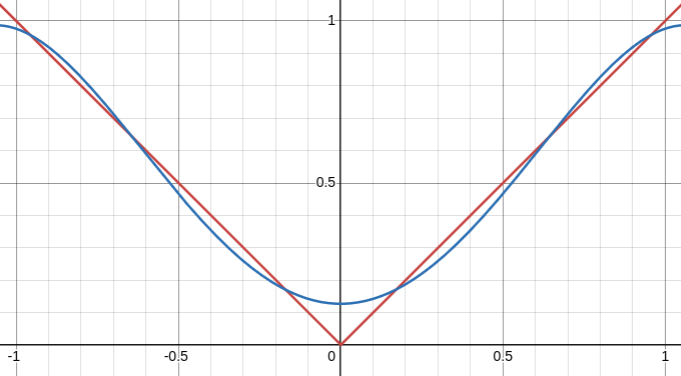
\includegraphics[width=0.5\linewidth]{Aproksymacja_x.png}
    \caption{Wykres obrazujący aproksymację}
    \label{fig:aprox}
\end{figure}

\subsection*{Wnioski}

Jak widać na wykresie \ref{fig:aprox} i w tabeli \ref{tab:comparison}, aproksymacja jest naprawdę bliska oryginalnej funkcji. Jedynie w punkcie $x = 0$, gdzie błąd względny wynosi $10 \%$, występuje znaczna różnica między funkcją a jej aproksymacją.

\section*{Zadanie 2}
\section*{Dane:}
Mamy dane: 
\[
(0.0,0.0),\quad (0.5,1.6),\quad (1.0,2.0),\quad (6.0,2.0),\quad (7.0,1.5),\quad (9.0,0.0).
\]

\section*{(a) Wielomian interpolacyjny stopnia 5}
Wiedząc, że dla \( n+1 \) punktów (tutaj \( n+1 = 6 \)) istnieje jedyny wielomian stopnia co najwyżej \( n=5 \), szukamy \( P_5(x) \) w postaci:
\[
P_5(x) = a_0 + a_1 x + a_2 x^2 + a_3 x^3 + a_4 x^4 + a_5 x^5.
\]
Współczynniki \( a_0, a_1, \ldots, a_5 \) wyznaczamy z układu równań wynikającego z warunku:
\[
P_5(x_i) = y_i,\quad i=1,\ldots,6.
\]
Przykładowo:
\[
\begin{cases}
a_0 + a_1\cdot 0.0 + a_2\cdot 0.0^2 + \dots + a_5\cdot 0.0^5 = 0.0,\\[1mm]
a_0 + a_1\cdot 0.5 + a_2\cdot (0.5)^2 + \dots + a_5\cdot (0.5)^5 = 1.6,\\[1mm]
a_0 + a_1\cdot 1.0 + a_2\cdot (1.0)^2 + \dots + a_5\cdot (1.0)^5 = 2.0,\\[1mm]
\vdots\\[1mm]
a_0 + a_1\cdot 9.0 + a_2\cdot (9.0)^2 + \dots + a_5\cdot (9.0)^5 = 0.0.
\end{cases}
\]

Do rozwiązania tego układu równań skorzystałem z bibliotecznej funkcji \texttt{numpy.linalg.solve}.

\begin{figure}[H]
    \centering
    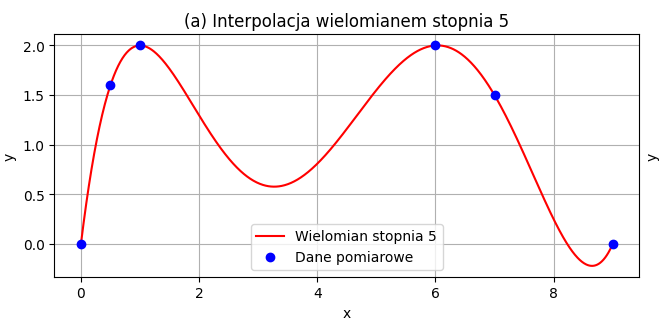
\includegraphics[width=1\linewidth]{Interpolacja_Wielomian_5_stopnia.png}
    \caption{Interpolacja punktów wyniku eksperymentu wielomianem piątego stopnia}
    \label{fig:interpol_5}
\end{figure}

\bigskip

\section*{(b) Funkcja sklejana stopnia trzeciego (spline)}
Kolejnym podejściem jest interpolacja przy użyciu sklejań kubicznych. \cite{wiki:Cubic_Spline,wiki:Spline_(mathematics)} W metodzie tej szukamy funkcji \( S(x) \) złożonej z kawałków wielomianów trzecich:
\[
S(x) = S_i(x),\quad x\in [x_i,x_{i+1}],\quad i=1,\ldots,5,
\]
gdzie każdy \( S_i(x) \) ma postać:
\[
S_i(x) = a_i + b_i (x-x_i) + c_i (x-x_i)^2 + d_i (x-x_i)^3.
\]
Warunki na sklejenie:
\begin{enumerate}
    \item Warunki interpolacji: 
    \[
    S_i(x_i) = y_i,\quad S_i(x_{i+1}) = y_{i+1}.
    \]
    \item Ciągłość pierwszej i drugiej pochodnej w punktach \( x_2, \ldots, x_5 \):
    \[
    S_i'(x_{i+1}) = S_{i+1}'(x_{i+1}),\quad S_i''(x_{i+1}) = S_{i+1}''(x_{i+1}).
    \]
    \item Dodatkowo przyjmujemy warunki brzegowe. Dla naturalnego splajn'u przyjmujemy:
    \[
    S_1''(x_1) = 0,\quad S_5''(x_6) = 0.
    \]
\end{enumerate}
Rozwiązując układ równań dla współczynników \( a_i, b_i, c_i, d_i \), uzyskujemy funkcję sklejaną \( S(x) \), która gładko interpoluje dane. \\

\begin{figure}[H]
    \centering
    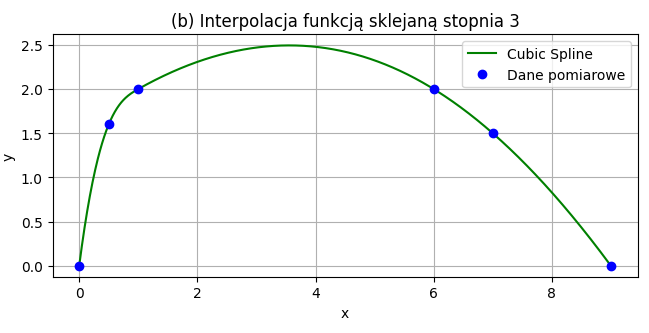
\includegraphics[width=1\linewidth]{spline_3_stopnia.png}
    \caption{Spline wielomianami trzeciego stopnia}
    \label{fig:spline}
\end{figure}

\bigskip

\section*{(c) Interpolacja przy pomocy wielomianów Czebyszewa}
Interpolacja przy użyciu wielomianów Czebyszewa polega na aproksymacji funkcji (lub danych) w bazie wielomianów Czebyszewa \( T_k(x) \).  
Rozważamy rozwinięcie funkcji \( f(x) \) (lub interpolanta \( P(x) \)) w szereg:
\[
P(x) = \sum_{k=0}^{n} c_k \, T_k(x),
\]
gdzie współczynniki \( c_k \) są wyznaczane na podstawie równań wynikających z warunków interpolacji. \\[1mm]


\begin{figure}[H]
    \centering
    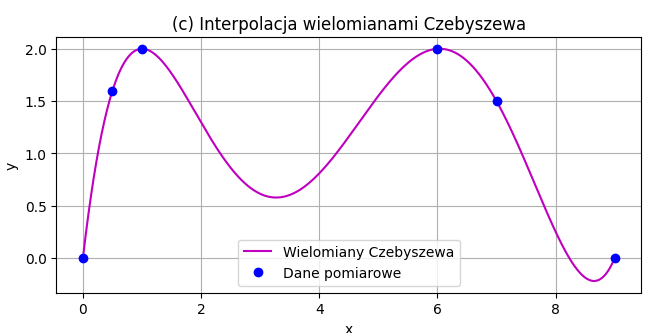
\includegraphics[width=1\linewidth]{Wielomiany_Czebyszewa.png}
    \caption{Wykres obrazujący interpolację punktów metodą Czebyszewa}
    \label{fig:cheby}
\end{figure}

\bigskip

\section*{(d) Porównanie wyników interpolacji}
\textbf{Wielomian stopnia 5:}  
Interpolant ten dokładnie przechodzi przez wszystkie punkty. Jednakże, przy nierównomiernym rozkładzie węzłów, może wystąpić zjawisko oscylacyjne (efekt Rungego), zwłaszcza na krańcach przedziału, co może skutkować nienaturalnym przebiegiem między punktami.

\medskip

\textbf{Spline wielomianu stopnia trzeciego:}  
Sklejana funkcja interpolacyjna jest składana kawałkami – dla każdego przedziału \( [x_i, x_{i+1}] \) mamy oddzielny wielomian. Dzięki warunkom ciągłości pierwszej i drugiej pochodnej uzyskujemy gładką krzywą, która zazwyczaj nie wykazuje widocznych oscylacji między punktami. Zaletą tego podejścia jest lokalny charakter – zmiana wartości w jednym przedziale nie wpływa na całą funkcję.

\medskip

\textbf{Interpolacja z bazą wielomianów Czebyszewa:}  
Gdybyśmy mieli możliwość wyboru węzłów, metoda Czebyszewa pozwala na konstrukcję interpolanta o mniejszych oscylacjach dzięki optymalnemu rozmieszczeniu punktów (węzłów Czebyszewa minimalizują tzw. stałą Lebesgue’a). W naszym zadaniu, o ile dokonamy odpowiedniej transformacji, możemy uzyskać interpolanta, który jest numerycznie stabilniejszy niż bezpośredni wielomian interpolacyjny wyższego stopnia, ale – przy zadanych eksperymentalnych punktach – niekoniecznie da znaczącą poprawę względem splajnów.

\medskip

\textbf{Wnioski:}  
Najlepszym podejściem dla danych eksperymentalnych jest zazwyczaj interpolacja przy użyciu \textbf{spline’ów} (punkt (b)), ponieważ:
\begin{itemize}
    \item \textbf{Lokalność:} Sklejany interpolant (spline) jest tworzony lokalnie – błąd w jednym przedziale nie przenosi się na inne.
    \item \textbf{Brak oscylacji:} W przeciwieństwie do globalnego wielomianu stopnia 5, spline nie generuje niepożądanych oscylacji między punktami.
    \item \textbf{Gładkość:} Zapewnienie ciągłości pierwszej i drugiej pochodnej prowadzi do bardziej naturalnego przebiegu krzywej, co jest często pożądane w interpretacji wyników eksperymentalnych.
\end{itemize}
Oczywiście metoda interpolacji przy użyciu wielomianów Czebyszewa ma duże zalety w aproksymacji funkcji (szczególnie gdy można wybrać optymalne węzły), jednak przy takich danych – gdy punkty są już danymi pomiarowymi – spline zazwyczaj daje bardziej „realistyczny” przebieg krzywej.

\begin{figure}[H]
    \centering
    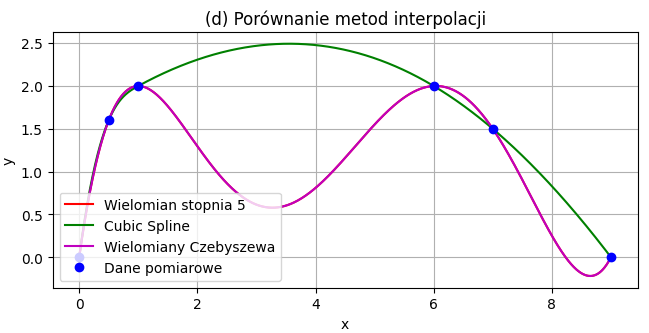
\includegraphics[width=1\linewidth]{Zestawienie.png}
    \caption{Wykres zestawiający wszystkie podejścia}
    \label{fig:all}
\end{figure}

\section*{Implementacja skryptu generująca powyższe wykresy}

Poniżej znajduje się pełny skrypt generujący wykresy \ref{fig:interpol_5}, \ref{fig:cheby}, \ref{fig:spline} i \ref{fig:all}

\begin{verbatim}
    import numpy as np
import matplotlib.pyplot as plt
from scipy.interpolate import CubicSpline
from numpy.polynomial.chebyshev import chebfit, chebval

# Experimental data
x_data = np.array([0.0, 0.5, 1.0, 6.0, 7.0, 9.0])
y_data = np.array([0.0, 1.6, 2.0, 2.0, 1.5, 0.0])

# Points to be ploted 
x_plot = np.linspace(0, 9, 1000)

def polynomial_interpolation(x, y):
    A = np.vstack([x**i for i in range(6)]).T
    coeffs = np.linalg.solve(A, y)
    
    def poly_func(x_new):
        result = np.zeros_like(x_new, dtype=float)
        for i, coeff in enumerate(coeffs):
            result += coeff * (x_new ** i)
        return result
    
    return poly_func, coeffs

def cubic_spline_interpolation(x, y):
    spline = CubicSpline(x, y)
    return spline

def chebyshev_interpolation(x, y, degree=5):
    x_scaled = 2 * (x - np.min(x)) / (np.max(x) - np.min(x)) - 1
    
    coeffs = chebfit(x_scaled, y, degree)
    def cheb_func(x_new):
        x_new_scaled = 2 * (x_new - np.min(x)) / (np.max(x) - np.min(x)) - 1
        return chebval(x_new_scaled, coeffs)
    
    return cheb_func, coeffs

poly_func, poly_coeffs = polynomial_interpolation(x_data, y_data)
spline_func = cubic_spline_interpolation(x_data, y_data)
cheb_func, cheb_coeffs = chebyshev_interpolation(x_data, y_data)

y_poly = poly_func(x_plot)
y_spline = spline_func(x_plot)
y_cheb = cheb_func(x_plot)

plt.figure(figsize=(15, 10))

# Polynomial interpolation
plt.subplot(2, 2, 1)
plt.plot(x_plot, y_poly, 'r-', label='Wielomian stopnia 5')
plt.plot(x_data, y_data, 'bo', label='Dane pomiarowe')
plt.title('(a) Interpolacja wielomianem stopnia 5')
plt.xlabel('x')
plt.ylabel('y')
plt.grid(True)
plt.legend()

# Spline
plt.subplot(2, 2, 2)
plt.plot(x_plot, y_spline, 'g-', label='Cubic Spline')
plt.plot(x_data, y_data, 'bo', label='Dane pomiarowe')
plt.title('(b) Interpolacja funkcją sklejaną stopnia 3')
plt.xlabel('x')
plt.ylabel('y')
plt.grid(True)
plt.legend()

# Chebyshev interpolation
plt.subplot(2, 2, 3)
plt.plot(x_plot, y_cheb, 'm-', label='Wielomiany Czebyszewa')
plt.plot(x_data, y_data, 'bo', label='Dane pomiarowe')
plt.title('(c) Interpolacja wielomianami Czebyszewa')
plt.xlabel('x')
plt.ylabel('y')
plt.grid(True)
plt.legend()

# Method comparison 
plt.subplot(2, 2, 4)
plt.plot(x_plot, y_poly, 'r-', label='Wielomian stopnia 5')
plt.plot(x_plot, y_spline, 'g-', label='Cubic Spline')
plt.plot(x_plot, y_cheb, 'm-', label='Wielomiany Czebyszewa')
plt.plot(x_data, y_data, 'bo', label='Dane pomiarowe')
plt.title('(d) Porównanie metod interpolacji')
plt.xlabel('x')
plt.ylabel('y')
plt.grid(True)
plt.legend()

plt.tight_layout()
plt.show()

print("Polynomial coefficients:")
for i, coeff in enumerate(poly_coeffs):
    x = f"x ^ {i}" if i > 0 else ''
    print(f"{round(coeff,10)} * {x} + ", end='')
print()

\end{verbatim}

\bigskip

\bibliographystyle{plain}
\bibliography{references}

\end{document}

